\documentclass[usenatbib]{mnras}
\usepackage[T1]{fontenc}
\usepackage{ae,aecompl}

\usepackage{graphicx}	% Including figure files
\usepackage{amsmath}	% Advanced maths commands
\usepackage{amssymb}	% Extra maths symbols
\usepackage{array}
\usepackage{physics}

\usepackage{multirow}
\usepackage{multicol}
\usepackage{blindtext}
\newcolumntype{?}{!{\vrule width 1pt}}
\newcommand{\Msun}{\,{\rm M}$_{\odot}$\,}
\newcommand{\Mpch}{\,{\rm Mpc}\,\ifmmode h^{-1}\else $h^{-1}$\fi}
\newcommand{\kpch}{\,{\rm kpc}\,\ifmmode h^{-1}\else $h^{-1}$\fi}
\newcommand{\kpc}{\,{\rm kpc}\,}
\newcommand{\kms}{\,{\rm km}\ s$^{-1}$\,}

%%%%%%%%%%%%%%%%%%% TITLE PAGE %%%%%%%%%%%%%%%%%%%
\title[Superclusters from velocity divergence fields]{Superclusters from velocity divergence fields}
\author[Pe\~naranda-Rivera et al.]{
\parbox[t]{\textwidth}{
    {J. D. Pe\~naranda-Rivera $^1$,} 
    {D. L. Paipa-Le\'on$^{1}$,}
    {S. D. Hern\'andez-Charpak$^{1,2}$,}\\
    {J. E. Forero-Romero $^{1}$}
}
\\\\
$^{1}$ Departamento de F\'isica, Universidad de los Andes, Cra. 1
  No. 18A-10 Edificio Ip, CP 111711, Bogot\'a, Colombia \\
$^{2}$ Center for Neuroprosthetics and Brain Mind Institute, Swiss
  Federal Institute of Technology (EPFL), CH-1015, Lausanne,
  Switzerland\\  
}

% These dates will be filled out by the publisher
\date{Accepted XXX. Received YYY; in original form ZZZ}

% Enter the current year, for the copyright statements etc.
\pubyear{2019}


% Don't change these lines
\begin{document}
\label{firstpage}
\pagerange{\pageref{firstpage}--\pageref{lastpage}}
\maketitle

%%%%%====MYMARK========
\maketitle
\begin{abstract}
Galaxy superclusters can be defined as regions of converging galaxy
velocity flows. Such structures have quantifiable properties such as
mass, volume and shape. The most precise quantification of such an
object has been done on our local supercluster, Laniakea. In this work
the properties of Laniakea are compared to the expectations from a
$\Lambda$CDM Universe. Cosmological N-body simulations are used in
order to find cosmic flow fields of dark matter halos and find
superclusters using a watershed algorithm. In addition, the
distributions of volume of the superclusters found in those
simulations are quantified and compared with known values for
Laniakea. The latter process was done for both Planck 2015 cosmologies
and cosmologies with extreme values of $\Omega_m$ and $\sigma_8$
parameters. In all those cases Laniakea is found on the right side of
the distribution, placing it as an atypical object in a cosmological
context.  
\end{abstract}

\begin{keywords}
%%PREGUNTAR
%galaxies:supercluster --- simulation:cosmological --- filter:gaussian --- methods:numerical
\end{keywords}


%=========================================================================
%		PAPER CONTENT
%=========================================================================

%*************************************************************************

\section{Introduction}
% La introduccion y el abstract es lo ultimo que se escribe.


In 2014 astronomers used a peculiar velocities map  to 
define the Laniakea supercluster of galaxies
\citep{2014Natur.513...71T}.  
Their main input was the Cosmicflows-2 catalog of distances and radial
velocities that provide them with coverage of distances up to 400 Mpc
[CITA A COSMICFLOWS-2]. 
By applying a Wiener filter \citep{Zaroubi_1999} they obtained the
reconstruction of the 3-dimensional velocity field. 
From this reconstructions they our local galaxy supercluster, Laniakea.
Laniakea thus represents the region of inflowing peculiar velocities
that include the Milky Way. 
The volume spanned by Laniakea is close to isotropic with an 
approximate diameter of $160$ Mpc encompassing a mass of
$\approx 10^{17}$ \Msun.

From a general computational point of view the definition of Laniakea poses
an interesting problem, namely defining regions of converging velocity
flows.
This conceptual statement has been recently exploited by \cite{Dupuy_2019} 
to use streamlines found in peculiar velocity data and find
superclusters. 
They make use of the concept of basins of attraction/repulsion, defined as
regions where velocity flows are observed to be inflowing/outflowing
as consequence of gravitational forces. 
In practice, they track streamlines in space to define gravitational
basins of attraction/repulsion.   

\cite{Dupuy_2020} studied in detail the influence of the details in
the algorithm parameters in the detected gravitational basins. 
The computation of the streamlines involves the application of a
fourth order Runge-Kutta method. 
In this way, obtaining structures using this method is influenced by
the choice of the integration parameters. 
The interpretation of basins of attraction or repulsion
also depends on the direction in which the integration is carried
out. 

Additionally, the
influence of a smoothing parameter (named smoothing scale) is also a
focus of interest in the latter work, and the results found are
expected to be the same in this paper. 

In this paper we are interested in superclusters, which are defined as
the union of the elements of the cosmic network that form an
identifiable structure. 
Studying this type of structures involves the
same difficulties of studying the cosmic web as they are not found by
a unique method. In particular, luminosity density data has been one
of the selected ways to find and classify superclusters in
observational data, as presented in \cite{Lietzen_2016} and
\cite{Bagchi_2017}. In addition, numerical simulations represent a
powerful tool in the study of superclusters as they allow investigators to
test different cosmological parameters and also to consider the time
evolution of the cosmic web components
\citep{Einasto_2019,einasto2020evolution}. Our main interest remains
in a kinematic approach to this problem, which will let us introduce a
supercluster finding algorithm that uses the divergence of the
velocity field of DM halos. 



The research developed by \cite{2014Natur.513...71T} corresponds to a kinematic approach to the problem of defining superclusters in observational data. 


In the same way, a joint work between the
observations and the simulations has been carried out in order to
fully understand this pattern in the universe. We can find an example
of the observational approach in \cite{Kim_2016}, where the
filamentary structures surrounding the Virgo cluster are analysed
using data from the HyperLeda database. 
Other examples of this
approach can be found in \cite{Santiago_Bautista_2020},
\cite{van_de_Weygaert_2014} and \cite{Lares_2017}. Finally, a
computational approach is presented in
\cite{10.1111/j.1365-2966.2009.14885.x} where a dynamical
classification of the cosmic web is applied to cosmological N-body
simulations.  

We aim to quantify if Laniakea can be considered as a typical or atypical 
structure in our current cosmological context. In order to achieve
this objective, we will apply a watershed algorithm
\citep{BeucherWatershed1979} which runs over the divergence field of
the velocity and segments the simulations used into isolated
groups. The process of structure finding using watershed methods is
explored in \cite{10.1111/j.1365-2966.2007.12125.x} where a extensive
analysis is made to connect image processing with astrophysics. In
particular, we will implement a watershed by immersion algorithm,
which depends only on the values of the divergence field.  

The following discussion presents a general approach to the
methodology to be used in the work, as well as the results found. In
this way, section 2 presents the numerical tools used, including the
operation of the finder algorithm, and section 3 presents the results
found after applying our method to different simulations. 




\section{Auto-correlation length in the divergence field}

We use the velocity divergence field, $\div \textbf{v}$, as the main quantity to study over cosmological scales.
From it we define a dimensionless divergence field, $\delta(\textbf{r})$, as follows:

\begin{equation}
    \delta (\textbf{r})\equiv -\frac{1}{H_0 f} \div \bf{v},
    \label{eq:div}
\end{equation}
where $H_0$ is the Hubble parameter and $f$ is the growth rate of structure.
This is a purely computational definition motivated by the linear theory of structure formation where the equality between the two sides of Equation (\ref{eq:div}) is expected to actually hold.

We compute the power spectrum of this scalar field and denote it as $P_{\delta}(k)$. 
From this power spectrum we calculate the auto-correlation function as
\begin{equation}
    \xi_{\delta\delta} (r) = \frac{1}{2\pi^2}\int_{0}^{\infty} k^2 P_{\delta}(k)\frac{\sin kr}{kr} dk.
\end{equation}

From the auto-correlation function we define a coherence length, $R_{\delta\delta}$ as the value of $r$ at which $\xi_{\delta\delta}(r)$ drops by a factor of then from the value it has for $r\rightarrow0$. 
Computationally speaking, we compute the auto-correlation function in the interval $1\Mpch \leq r \leq 100 \Mpch$ and $R_{\delta\delta}$ is defined by the value at which
\begin{equation}
\xi_{\delta\delta}(R_{\delta\delta})  =\frac{1}{10} \xi_{\delta\delta}(1 \Mpch).    
\end{equation}

We show in the following sections how using this definition we obtain a linear relationship between the auto-correlation length, $R_{\delta\delta}$, and the average super-cluster size.


\begin{table*}
\begin{tabular}{c c c c c}\hline
Field &  $v_{max}$ & $L_b$ & $R_s$ & $N_c$\\
type & (km s$^{-1}$) & (\Mpch) & (\Mpch) & \\\hline
N-body & $150$ & $720$ & \{$6$, $12$, $30$, $48$, $60$\} & $120$\\
N-body & $200$ & $720$ & \{$5$, $10$, $20$, $30$, $40$\} & $144$\\
N-body & $300$ & $720$ & \{$2$, $6$, $10$, $14$, $20$\} & $360$\\
Gaussian & - & $720$ & \{$2$, $6$, $10$, $14$, $20$\} & $360$\\
Gaussian & - & $300$ & \{$3$, $9$, $12$, $15$, $18$\} & $100$\\
Gaussian & - & $1000$ & \{$10$, $15$, $20$, $30$, $40$\} & $100$\\\hline
\end{tabular}
\caption{Summary of the $30$ different dimensionless divergence fields used in this Letter. 
The Field type describes whether the field comes from the Abacus Simulations (N-body) or it is generated from the power spectrum (Gaussian). $v_{max}$ only applies to the N-body fields and refers to the minimum value of a halo maximum circular velocity to include it in the peculiar velocity field interpolation.
$L_b$ is the box size of the cubic volume used to compute the divergence. $R_{s}$ lists the gaussian smoothing (in the case of N-body fields) and the wavelength $1/R_s$ used to truncate the power spectrum (in the case of Gaussian fields). $N_c$ is the number of grid cells on a side of the interpolated density field.}
\label{table:values}
\end{table*}


\begin{figure*}
    \centering
    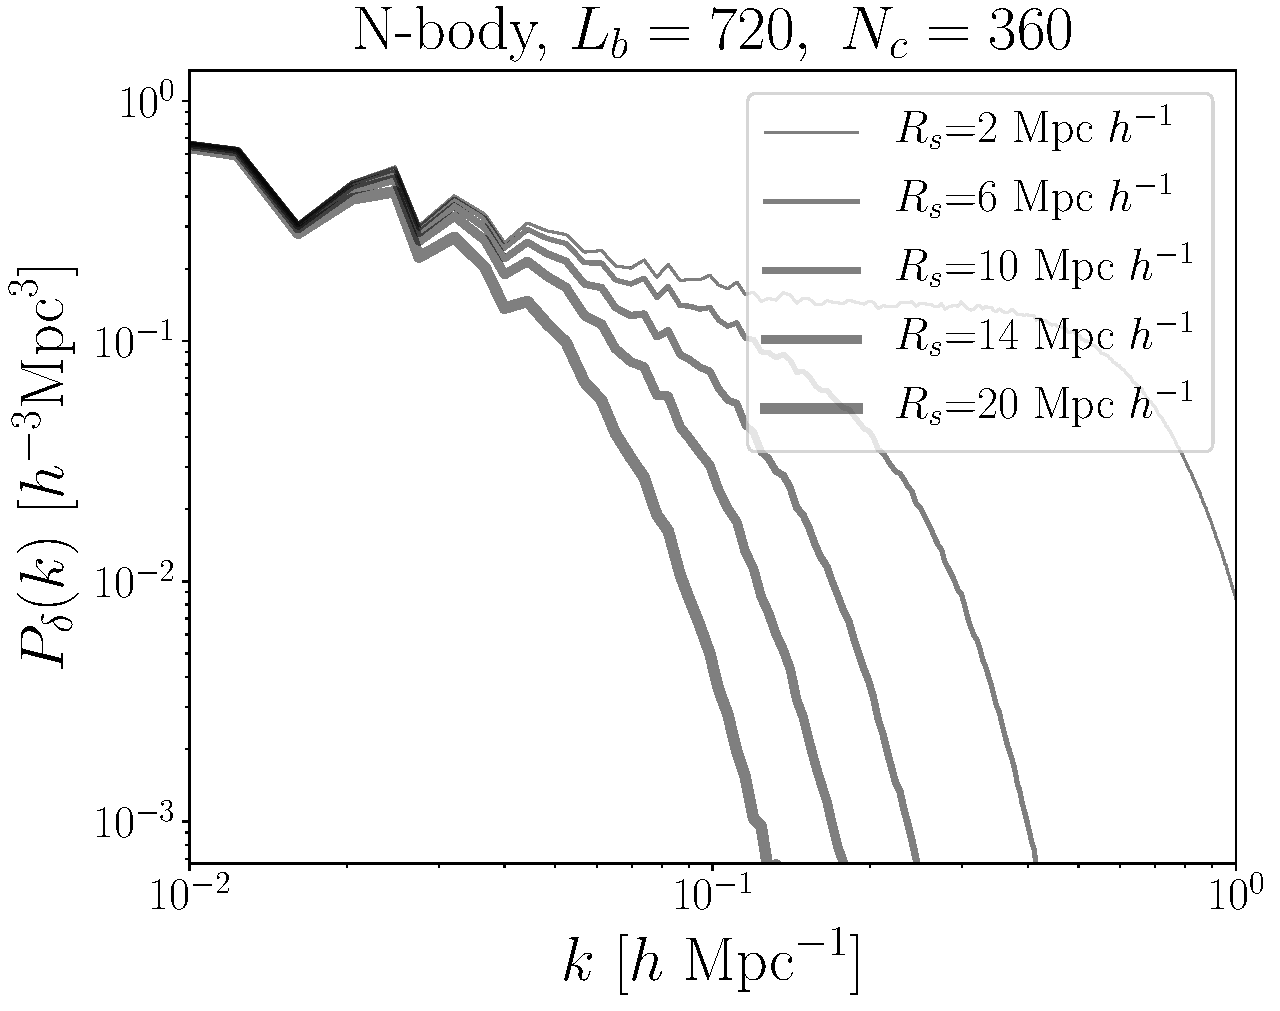
\includegraphics[width=240pt]{power_spectrum_nbody_720_360.pdf}
    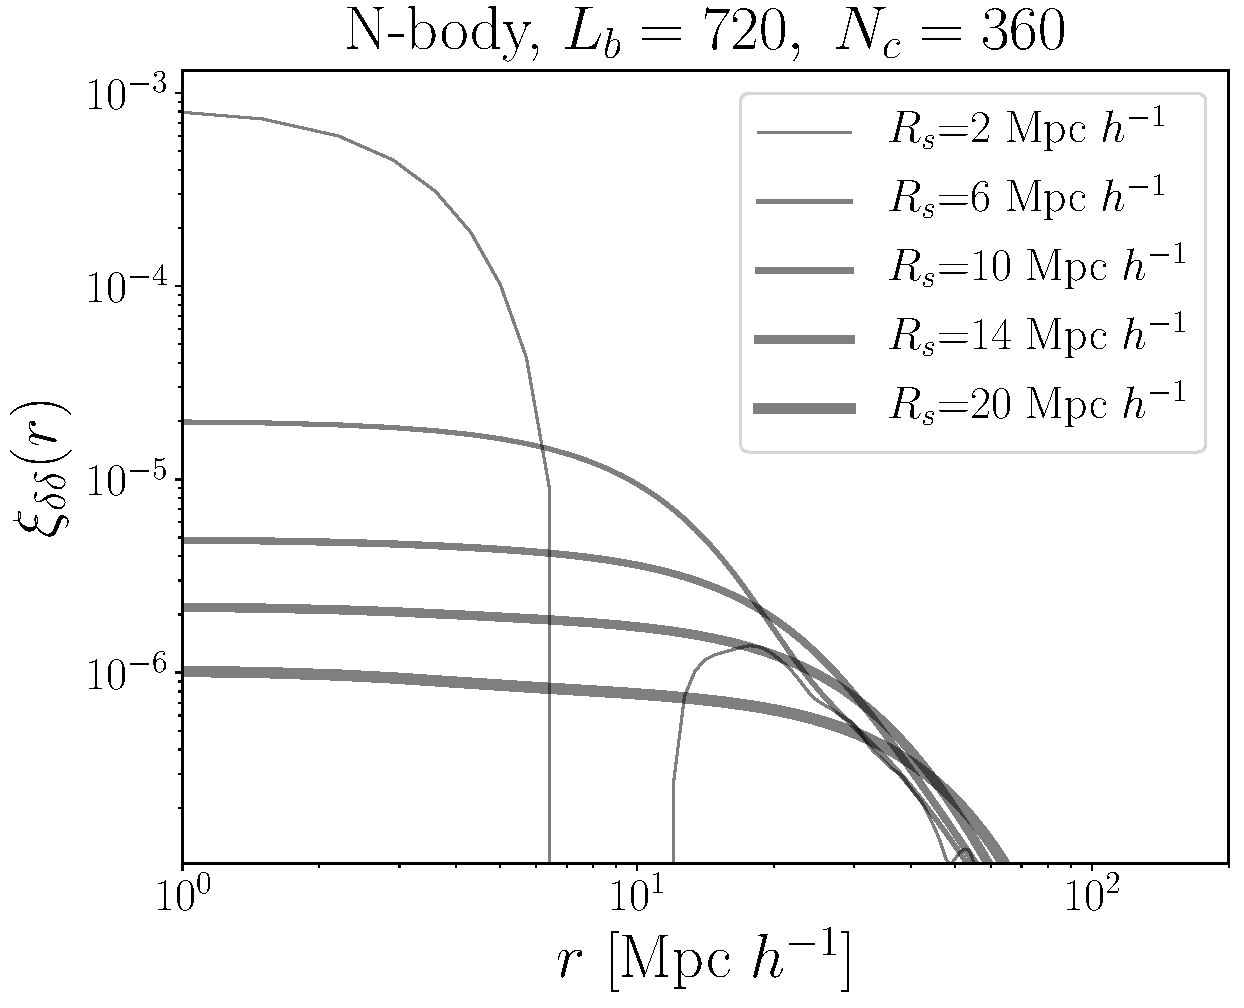
\includegraphics[width=240pt]{corr_func_nbody_720_360.pdf}
    \caption{Power spectrum (left) and auto-correlation function (right) for one of the $\delta$ fields computed using velocity interpolation from N-body data.
    The size of the cubic box is $L_b=720$ \hMpc and the number of voxels is $360^3$.
    Only dark matter haloes with maximum circular velocity larger than $300$ \kms were included in the velocity interpolation.
    Each line corresponds to a different Gaussian smoothing with length scale $R_s$.}
    \label{fig:nbody}
\end{figure*}

\begin{figure*}
    \centering
    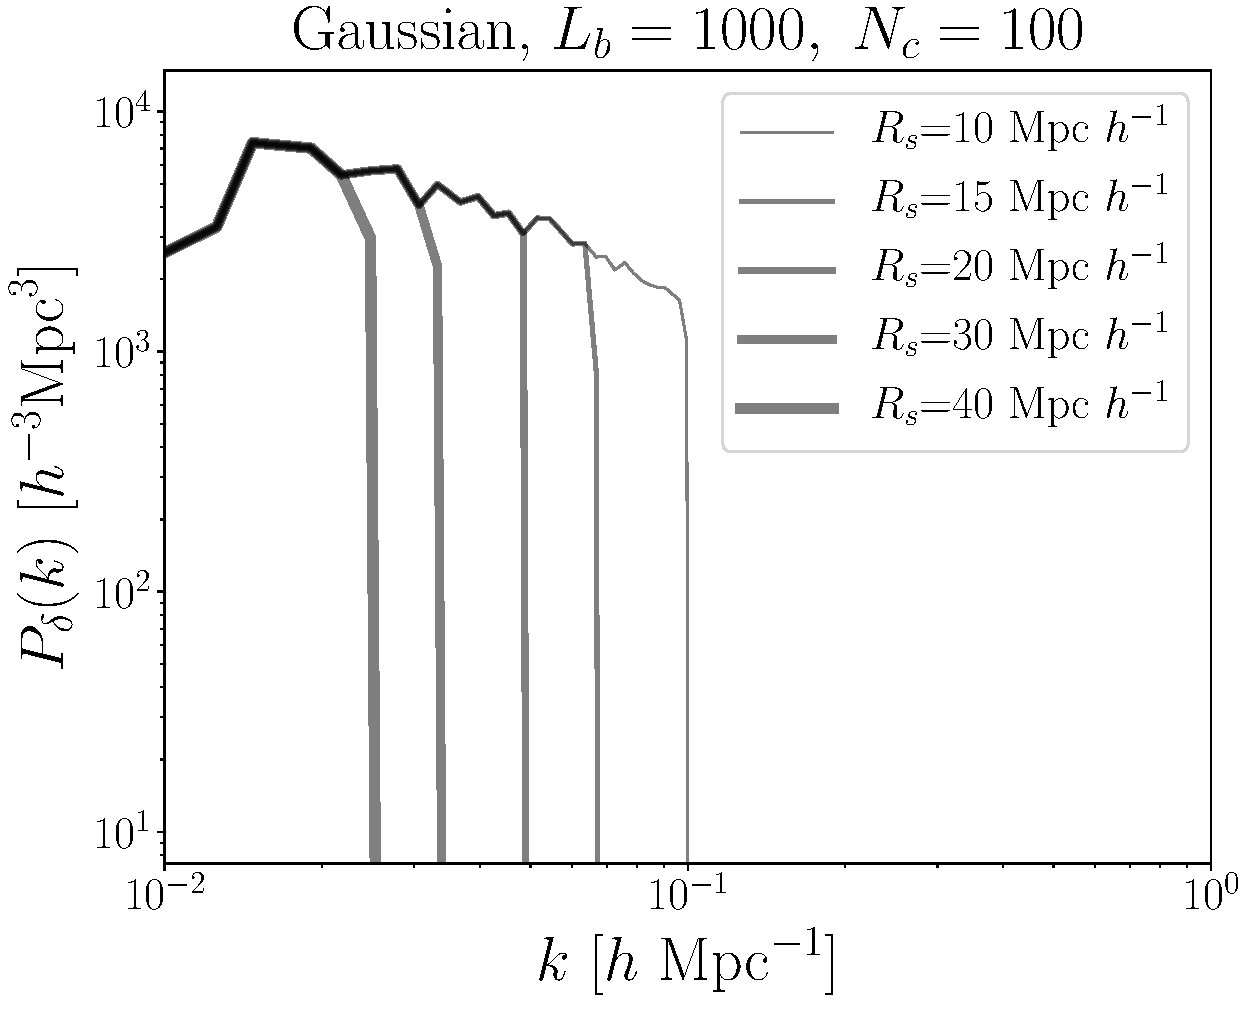
\includegraphics[width=240pt]{power_spectrum_gauss_1000_100.pdf}
    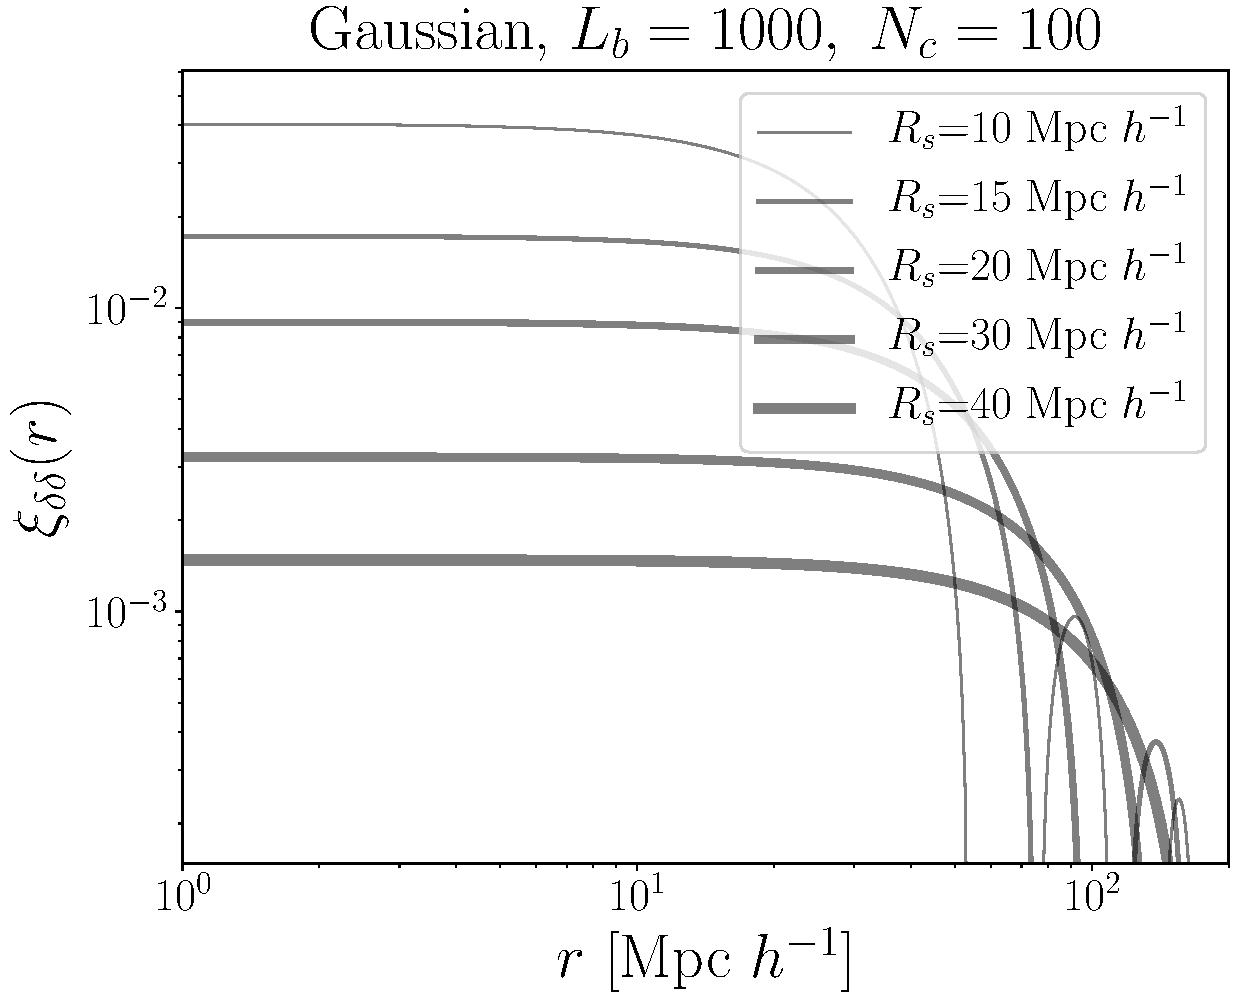
\includegraphics[width=240pt]{corr_func_gauss_1000_100.pdf}
    \caption{Power spectrum (left) and auto-correlation function (right) for one of the $\delta$ fields computed from linearly extrapolated power spectrum
    The size of the cubic box is $L_b=1000$ \hMpc and the number of voxels is $100^3$.
    Each line corresponds to a different truncation wavelength in the power spectrum of $1/R_s$.}
    \label{fig:gaussian}
\end{figure*}


\section{Divergence Fields on a Grid}
\label{sec:numerical_setup}

We use dimensionless divergence fields computed on a cubic grid. 
We generate them in two different ways.
The first corresponds to Gaussian fields with a truncated power spectrum coming from linear theory.
The second kind are fields generated by interpolation of biased tracers and smoothed with a Gaussian filter, with the tracers coming from N-body cosmological simulations.
In both cases the cosmological parameters correspond to the
$\Lambda$CDM Planck 2015 cosmology. 
We use a total of $30$ different divergence fields, summarized in Table \ref{table:values}, generated as follows.

\subsection{Gaussian fields with truncated power Spectrum}

We start by generating a density field with a power spectrum that follows no-wiggle parameterization of \cite{1998ApJ...496..605E}.
The power spectrum is extrapolated at $z=0$ using linear theory and truncated at $k_{\rm max}=1/R_s$.
This density field is generated over a cubic grid with $N_c^3$ cells over a cube of length $L_s$ on a side.
From this Gaussian density field we compute both $\delta(\textbf{r})$ and $\div \textbf{v}$.
We generate $15$ different Gaussian fields by changing the values for $L_b$, $N_c$ and $R_s$. 
Table \ref{table:values} summarizes the different values for those parameters.

\subsection{N-body fields from biased tracers with Gaussian smoothing}

We use the public Friend-of-Friends catalogs at redshift $z=0.1$
from the Abacus Project simulations to interpolate the haloes' peculiar velocity over a grid with $N_s^3$ cells.
The simulations were performed on a cube of side length $720$\ \Mpch with
$1440^3$ particles, corresponding to a DM particle mass resolution of $\sim 1 \times 10^{10}$ \Msun.
We start by selecting haloes with maximum circular velocity larger
than $v_{max}$.
Then we assign to each cell the value of the average velocity of the haloes in that cell, which is equivalent to a Nearest Grid Point interpolation scheme. 
If the cell is empty we assign a value of $0$\kms.
After this interpolation step we smooth the velocity field using a Gaussian filter of physical scale $R_s$.
We generate $15$ different N-body based divergence fields by changing the values for $v_{max}$, $N_c$ and $R_s$. 
Table \ref{table:values} summarizes the different values for those parameters.


\section{Watershed Superclusters}

We find the superclusters using a watershed algorithm \citep{BeucherWatershed1979} on the velocity divergence field.
The algorithm segments the whole volume by assigning each voxel to a unique supercluster. 

Our implementation works as follows. 
We sweep the cells in the divergence grid from the lowest values to the highest, i.e. from the high density regions with converging flows to the lowest density regions with divergent flows.
For the $i$-th cell under consideration we check whether its 26 neighbors have already been assigned to a group. 
If all the neighbors are unassigned, then this $i$-th cell starts a new group; if the majority of already assigned cells belongs to the $n$-th group, then this cell belongs to that group.
In case of a draw between groups, the cell is assigned to the supercluster with the lowest $n$ value.
At the end of the sweep all cells have been assigned to a group. 
In all our calculations we take periodical boundary conditions into account.  

We highlight that, once the divergence field is provided, this algorithm
does not have free parameters based either on divergence, density or distance thresholds. 
Finally, each group found by the algorithm is interpreted as a supercluster 
with a volume, $V_s$, calculated by the total volume of the voxels belonging to it.
From the volume $V_s$ we compute the equivalent radius $R_{\rm eq}$, that is the radius of the sphere with the same volume, 
   $ R_{\rm eq} = \left(\frac{3}{4\pi}V_{s}\right)^{1/3}$.
We describe the supercluster population in a divergence field by the average value of the equivalent radius, $\langle R_{\rm eq}\rangle$.


\section{Results}


The corresponding power spectra and autocorrelation function are presented in the right panel of Figure \ref{fig:power_spectrum}
 and Figure \ref{fig:autocorrelation}, respectively.
 
 
 

\begin{figure}
    \centering
    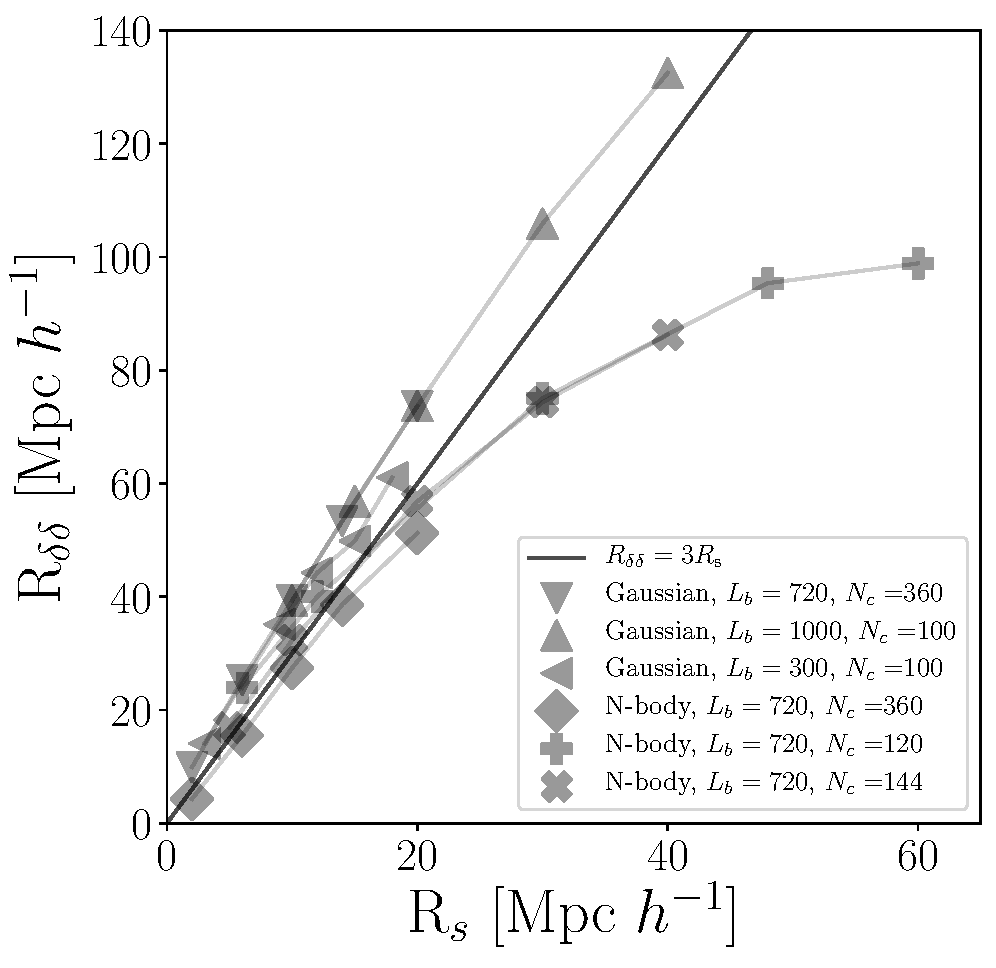
\includegraphics[width=240pt]{correlation_length.pdf}
    \caption{Correlation length $R_{\delta\delta}$ as a function of the truncation scale $R_s$.
    Both for Gaussian and N-body fields the relationship between the two scales is close to linear below $R_{s}=20$ \Mpch.}
    \label{fig:correlation length}
\end{figure}

 
\begin{figure}
    \centering
    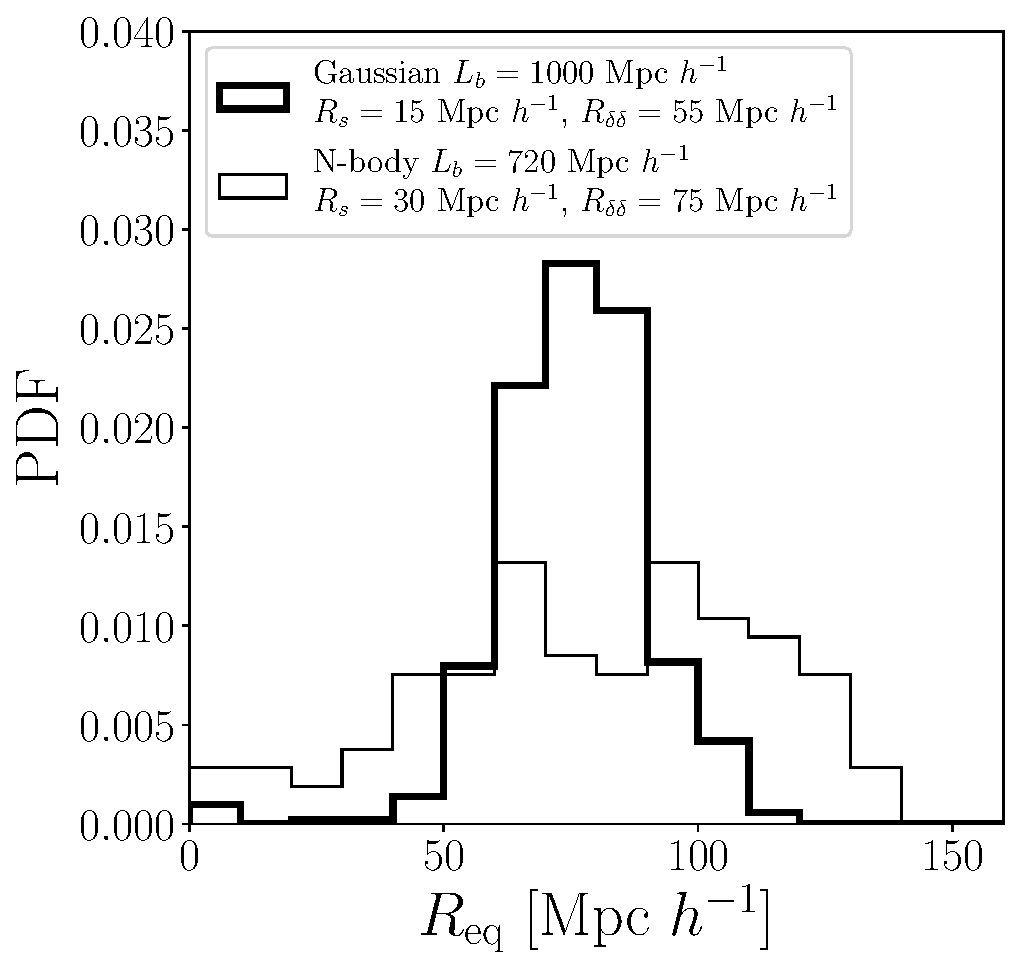
\includegraphics[width=240pt]{sizes_histogram.pdf}
    \caption{Equivalent radius distributions for a Gaussian Field and a N-body field.
    In both cases the average value for the equivalent radius are close to $80$\Mpch. 
    The shapes are different; the Gaussian field produces a narrower, closer to Gaussian, distribution than the N-body field. }  
    \label{fig:Nclusters}
\end{figure}


\begin{figure*}
    \centering
    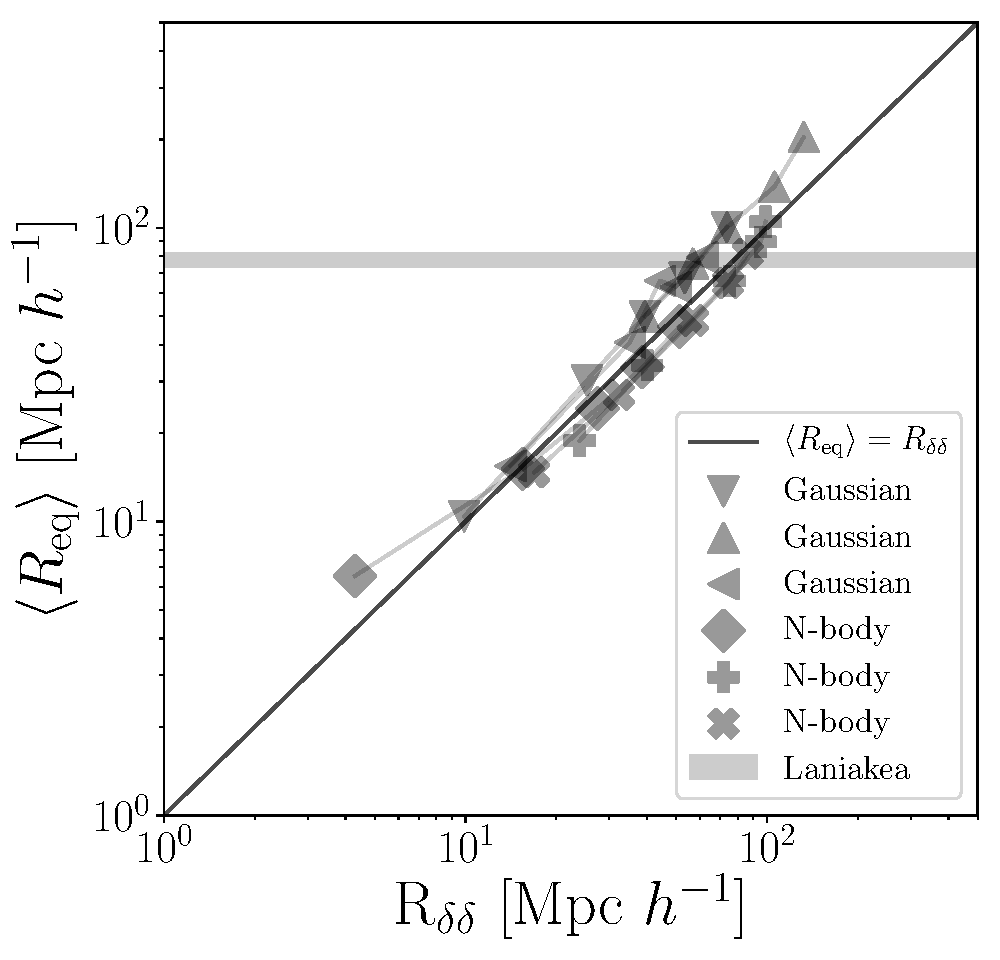
\includegraphics[width=330pt]{summary_watershed.pdf}
    \caption{Average equivalent radius as a function of the auto-correlation length in their parent divergence field.
    The relationship between the two quantities is close to linear for auto-correlation lengths below $100$ \Mpch. With the parameterization $\langle R_{\rm{eq}}\rangle=\alpha R_{\delta\delta}$, the best fit gives $\alpha=1.2\pm0.1$ for Gaussian fields and $\alpha=0.9\pm 0.1$ for N-body fields.
    \label{fig:Nclusters}.
    The horizontal stripe shows recent estimates of Laniakea's equivalent radius. If Laniakea is to be considered as an average supercluster, the the auto-correlation length in the divergence fields from the Cosmicflows data should be on the order of 65 to 90 \Mpch.}
\end{figure*}



\section{Discussion}

The selected superclusters has a significant dependence on the choice of $\sigma_s$. Therefore, if we want to compare the classification made by the algorithm with reported volume measures for Laniakea, we must choose wisely the value of the Gaussian length. Thus, the value reported by \cite{2014Natur.513...71T} in his studies on CosmicFlows-2 data is used. From now on, the value of the Gaussian length is fixed and equals 10\Mpch. 



\cite{2015MNRAS.452.1052L} used the velocity reconstruction on cosmicflows-2 data, the same reconstruction used to define Laniake.
The paper includes a computation of the dimensionless shear tensor $\Sigma_{\alpha\beta}=-\frac{1}{2H_0}\left(\frac{\partial v_\alpha}{\partial r_\beta}+\frac{\partial v_\beta}{\partial v_\alpha}\right)$ where $\alpha$ and $\beta$ represent the three cartesian components of the velocity $v$ and the position $r$ and $H_0$ is the Hubble-Lema\^itre constant.
With this definition the trace of the shear tensor is equal to minus the divergence of the velocity field.


The authors say that the formal reconstruction for the Wiener Filter velocity reconstruction is $5$\Mpch and the derivatives are computed over scales of $2.5$\Mpch. 
We use these two values as a bracket to be used later at the moment of comparing our results against observations.

A second piece of evidence that help us to pin down the effective smoothing scale comes from their reports on the numerical values of the shear tensor eigenvalues.
The authors found that the trace of the dimensionless shear tensor at the Local Group and Cen A location to be $0.030$ and $0.015$, respectively. 
These values translate into $3.0$ and $1.5$ in units of km $h$ Mpc$^{-1}$ s$^{-1}$. 
In Section XX we show that the divergence distributions in our calculations with a similar order of magnitude values correspond to 
to smoothing scales smaller than $6$\Mpch.





\section{Conclusions}
\label{sec:conclusions}


Throughout this investigation the main objective was to find a way to classify the Laniakea structure using N-body simulations. Thus, we made use of the dark matter halos velocity field divergence for the classification of structures in space. In addition, in order to achieve a robust result, different cosmologies were used to obtain the final results of the project.


First, a clear influence of the $\sigma_s$ parameter was observed when performing the segmentation process of the spatial grid through the Watershed algorithm. The latter behavior is produced by a great variation on the divergence field once this parameter is changed, as seen in figures \ref{fig:smooth_grad_dist} and \ref{fig:std_smooth}. In particular, the higher the value of $\sigma_s$, the larger the size of the convergent galaxy flow structures found in the simulations. As a consequence, when applying the algorithm with a greater $\sigma_s$ it is found that the superclusters are larger (behavior presented in figure \ref{fig:1Pert}).

However, the correct value of $\sigma_s$ corresponds to a physical choice. In particular, a value approximately of 10\Mpch. Therefore, once this parameter is adjusted, our algorithm has no free parameters that affect the generated distribution. Moreover, in order to classify the structure of Laniakea, we decided to use two types of cosmologies. 

The first set of cosmologies used corresponds to a generally accepted set of cosmological parameters given by Planck 2015 study. The volume distributions generated using this set of simulations, shown in figure \ref{fig:planck}, gives us a first idea that Laniakea is an atypical supercluster in terms of its size. On the other hand, a set of simulations with different cosmological parameters was used to evaluate their impact on the distributions. In particular, simulations using extreme values of $\Omega_m$ and $\sigma_s$ were selected. The resulting volume distributions are presented in figure \ref{fig:diferentes}. The same behavior as in Planck 2015 simulations is observed. 

In conclusion, we point out that the algorithm used in effect allows an effective partition of the simulations using the divergence field. Furthermore, it worked properly to allow us classifying Laniakea as an atypical supercluster in a cosmological context.




\bibliographystyle{mnras}
\bibliography{references}



\end{document}
